\documentclass[a4paper, 10pt, titlepage]{article}
\usepackage[utf8]{inputenc}
\usepackage[top=32mm, right=24mm, left=24mm]{geometry}
\usepackage{indentfirst}
\usepackage{graphicx}
\usepackage[hidelinks]{hyperref}
\usepackage{caption}

\title{\textbf{ECSE-487 \\ COMPUTER ARCHITECTURE LABORATORY \\ Assignment \#2}}
\author{Andrei Purcarus Craciun \\ 260631911}
\date{February 13, 2017}

\begin{document}

\maketitle

\section{Introduction}

This report describes the implementation, simulation and synthesis of a frequency synthesizer, an FSK modulator and an analog waveform generator. It also describes the use of pipelining to increase the clock rate of a slow design.

\section{Ripple-carry Frequency Synthesizer}

The frequency synthesizer was designed as a simple accumulator circuit. An internal register holds the sum, which is incremented by an input signal frequency\_control every rising edge. The carry-out of the adder is then used as a pulse generator whose frequency is given by the overflow rate of the register, or
\[ f_{out} = frequency\_control * \frac{f_{clk}}{N} \]
for an N-bit register.

First, a full adder circuit was implemented. Then, N full adders were joined together inside of a ripple carry adder, which was made generic in order to simplify reuse. An N-bit register component was also designed, with the same generic features. Finally, these components were instantiated in a frequency synthesizer, which was also made generic. The carry-out of the adder was then delayed through a register in order to avoid hazards in the output that could occur during output transitions. These components are described in the following files:
\begin{itemize}
    \item full\_adder.vhd
    \item ripple\_carry\_adder.vhd
    \item register.vhd
    \item ripple\_frequency\_synthesizer.vhd
\end{itemize}

The module described above was instantiated in a test-bench with N = 5. A 64 MHz clock was used, and pulses with frequencies of 2 MHz, 4 MHz, 20 MHz, 22 MHz, 32 MHz and 62 MHz were generated, as shown in Figures \ref{fig:ripple_1}, \ref{fig:ripple_2} and \ref{fig:ripple_3}. As these figures show, the frequency synthesizer can only generate average frequencies, and the remainder left in the register after an overflow will eventually cause clock jitter if the frequency generated does not evenly divide the clock frequency (such as the 20 MHz and 22 MHz signals in Figure \ref{fig:ripple_2}). In addition, the 62 MHz signal in Figure \ref{fig:ripple_3} shows significant jitter, as is to be expected since the frequency is very close to the clock frequency.

\begin{figure}[!htb]
    \centering
    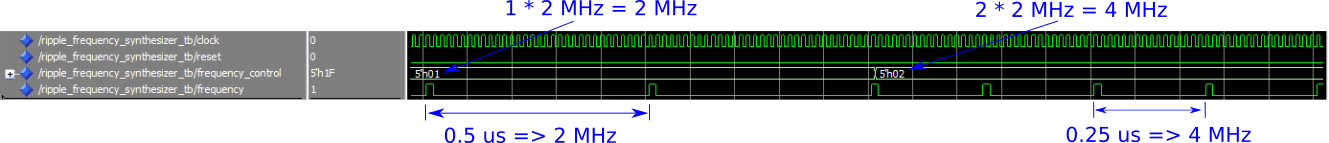
\includegraphics[width=\linewidth]{ripple_2_4_MHz.PNG}
    \caption{Frequencies of 2 MHz and 4 MHz generated by the ripple-carry frequency synthesizer.}
    \label{fig:ripple_1}
\end{figure}
\begin{figure}[!htb]
    \centering
    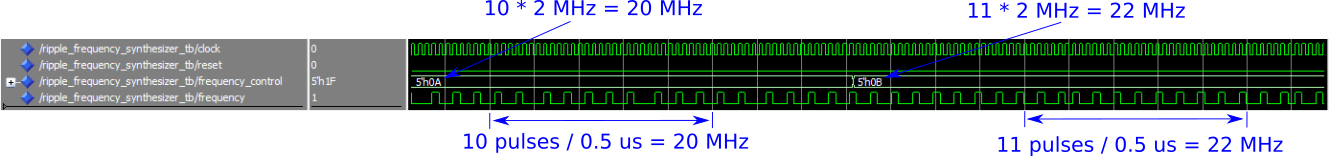
\includegraphics[width=\linewidth]{ripple_20_22_MHz.PNG}
    \caption{Frequencies of 20 MHz and 22 MHz generated by the ripple-carry frequency synthesizer.}
    \label{fig:ripple_2}
\end{figure}
\begin{figure}[!htb]
    \centering
    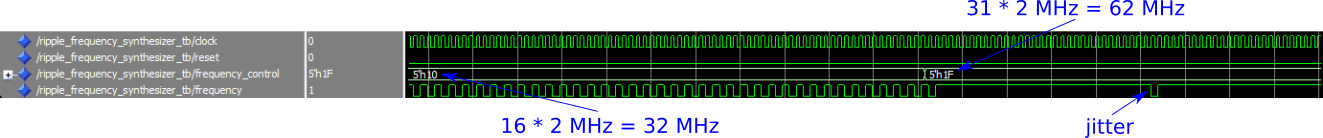
\includegraphics[width=\linewidth]{ripple_32_62_MHz.PNG}
    \caption{Frequencies of 32 MHz and 62 MHz generated by the ripple-carry frequency synthesizer. Note the significant jitter on the 62 MHz wave.}
    \label{fig:ripple_3}
\end{figure}

The circuit was then synthesized on a Cyclone V 5CSEMA5F31C6 FPGA in order to perform a timing analysis. Using generics, the timing analysis was performed for both N = 5 and N = 32. For N = 5, the result was a maximum clock rate of 142.71 MHz, and for N = 32, the result was a maximum clock rate of 112.23 MHz. These results are reasonable given the simplicity of the circuit and the nominal clock rate for this FPGA of 50 MHz.

\section{Pipelined Frequency Synthesizer}

In order to improve the clock rate found in the previous section, pipeline registers were added between the carry signals of the full adder components. In order to prevent phase discontinuity when the input changes, a pipeline was also added to the input in the form of a delay equalizer. This circuit makes the input change propagate along the pipeline at the same time as the final adder computation of the previous input, ensuring no sudden changes in output which would cause phase discontinuity. N of these building blocks were then instantiated to create a pipelined frequency synthesizer. These components are described in the following files:
\begin{itemize}
    \item accumulator.vhd
    \item delay\_equalizer.vhd
    \item bit\_slice.vhd
    \item pipelined\_frequency\_synthesizer.vhd
\end{itemize}

The module described above was instantiated with N = 5. A 64 MHz clock was used, and pulses with frequencies of 2 MHz, 4 MHz, 20 MHz, 22 MHz, 32 MHz and 62 MHz were generated, as shown in Figures \ref{fig:pipeline_1}, \ref{fig:pipeline_2} and \ref{fig:pipeline_3}.

\begin{figure}[!htb]
    \centering
    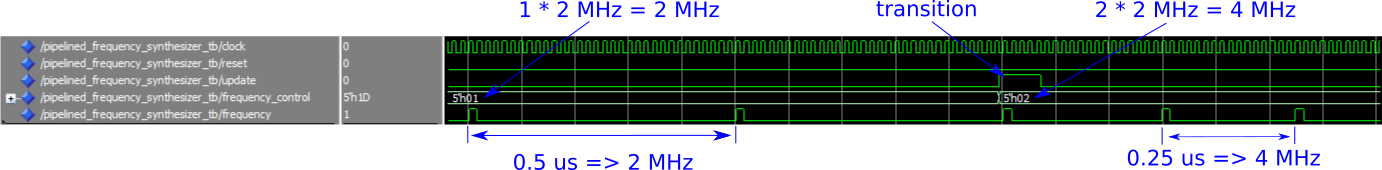
\includegraphics[width=\linewidth]{pipeline_2_4_MHz.PNG}
    \caption{Frequencies of 2 MHz and 4 MHz generated by the pipelined frequency synthesizer.}
    \label{fig:pipeline_1}
\end{figure}
\begin{figure}[!htb]
    \centering
    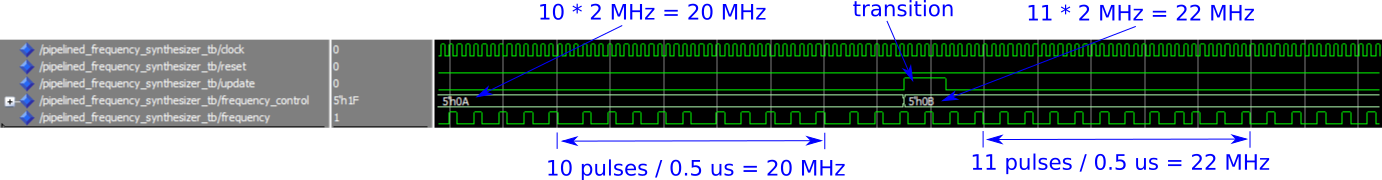
\includegraphics[width=\linewidth]{pipeline_20_22_MHz.PNG}
    \caption{Frequencies of 20 MHz and 22 MHz generated by the pipelined frequency synthesizer.}
    \label{fig:pipeline_2}
\end{figure}
\begin{figure}[!htb]
    \centering
    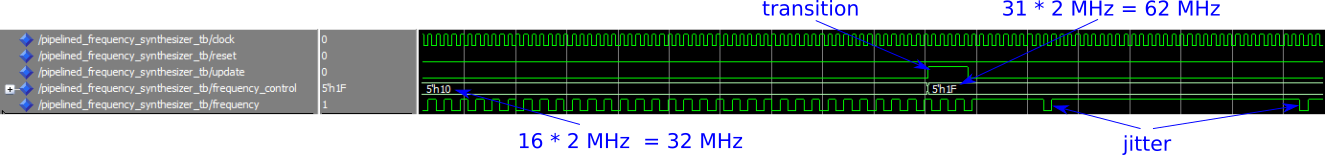
\includegraphics[width=\linewidth]{pipeline_32_62_MHz.PNG}
    \caption{Frequencies of 32 MHz and 62 MHz generated by the pipelined frequency synthesizer. Note the significant jitter on the 62 MHz wave.}
    \label{fig:pipeline_3}
\end{figure}

The circuit was then synthesized on a Cyclone V 5CSEMA5F31C6 FPGA in order to perform a timing analysis. Using generics, the timing analysis was performed for both N = 5 and N = 32. For N = 5, the result was a maximum clock rate of 149.37 MHz, and for N = 32, the result was a maximum clock rate of 144.01 MHz. The pipelined implementation resulted in an increase in the maximum clock rate for the circuit, as shown in Table \ref{tab:fmax}. For N = 5, the improvement is small, but it gets larger as N increases, as shown by the N = 32 case. This is because pipelining enables the propagation delay to stay roughly constant with increasing N, while the ripple-carry adders' propagation delay increases linearly with increasing N.

\begin{table}[!htb]
    \centering
    \begin{tabular}[c]{ l | c | c }
        & \textbf{N = 5} & \textbf{N = 32} \\
        \hline
        \textbf{ripple-carry} & 142.71 MHz & 112.23 MHz \\
        \hline
        \textbf{pipelined} & 149.37 MHz & 144.01 MHz \\
    \end{tabular}
    \caption{Maximum clock frequencies for the ripple-carry and pipelined implementations of the frequency synthesizer.}
    \label{tab:fmax}
\end{table}

\section{FSK Modulator}

The pipelined frequency synthesizer described above was then modified to produce an FSK modulator. First, the delay equalizer was modified to add a second input, and the propagating update signal was used to control which input gets loaded into the accumulator. If the update signal changes from a 1 to a 0, the first input gets loaded. If the update signal changes from a 0 to a 1, the second input gets loaded. Finally, if the update signal does not change between cycles, the output is unchanged. N of these new modules were then instantiated in the FSK modulator. The carry-out of the adder was then used as a toggle input for a T flip-flop, which generates output waveforms with half the frequency but 50-50 duty cycles. These components are described in the following files:
\begin{itemize}
    \item accumulator.vhd
    \item fsk\_delay\_equalizer.vhd
    \item fsk\_bit\_slice.vhd
    \item fsk\_modulator.vhd
\end{itemize}

The module described above was then instantiated with N = 5 and connected to inputs of 10 and 11 in order to generate the 10/11 MHz FSK modulation. A bit vector was then fed in to be modulated. The resulting modulation is shown in Figures \ref{fig:fsk_1} and \ref{fig:fsk_2}. These figures clearly show that the required frequencies are generated correctly, that no phase discontinuity occurs, and that the waveforms have 50-50 duty cycles. Due to the jitter problems described previously for these frequencies, the 50-50 duty cycles sometimes deviate slightly, which is to be expected given the design.

\begin{figure}[!htb]
    \centering
    \includegraphics[width=\linewidth]{fsk_10_11_MHz.PNG}
    \caption{FSK modulation of the nrz\_data signal with 10 MHz and 11 MHz square waves. Note the correct frequency generation.}
    \label{fig:fsk_1}
\end{figure}
\begin{figure}[!htb]
    \centering
    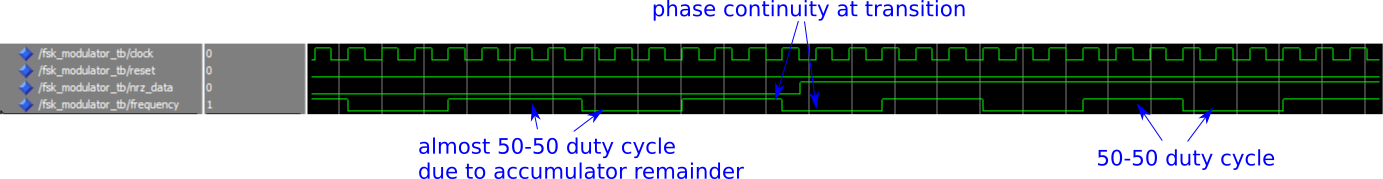
\includegraphics[width=\linewidth]{fsk_50-50_phase.PNG}
    \caption{FSK modulation of the nrz\_data signal with 10 MHz and 11 MHz square waves. Note the 50-50 duty cycle and the phase continuity during data changes.}
    \label{fig:fsk_2}
\end{figure}

\section{Analog Waveform Generator}

The pipelined frequency synthesizer described above was then used to implement an analog waveform generator. The pulse output of the synthesizer was used as an enable input for a 0-9 counter. This results in a counter that counts up once every period. The output of this counter was used as an address for a ROM, which was configured with the 8-bit amplitude of the signal
\[ 128 (1 + sin(\frac{2 \pi}{10} t)), t = 0, 1, \ldots 9 \]
Due to the counter, the frequency of the resulting wave is divided by 10 relative to the input frequency. This component is described in the following file:
\begin{itemize}
    \item analog\_waveform\_generator.vhd
\end{itemize}

The component was then instantiated with N = 5, and frequencies of 2 MHz, 4 MHz and 32 MHz were input. This resulted in sine waves with frequencies of 200 kHz, 400 kHz and 3.2 MHz, as shown in Figure \ref{fig:analog}. These frequencies were chosen as divisors of 64 MHz to avoid jitter in the output waveform. The simulation results also clearly show the lack of phase discontinuity more clearly than Figure \ref{fig:fsk_2}.

\begin{figure}[!htb]
    \centering
    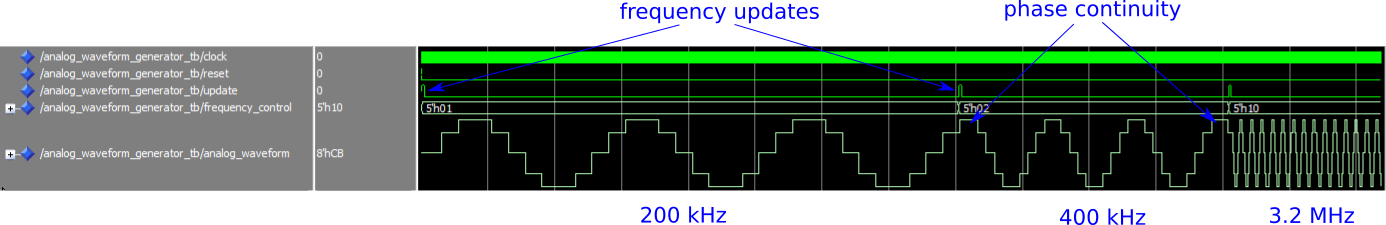
\includegraphics[width=\linewidth]{analog.PNG}
    \caption{Analog waveform generation of sine waves at frequencies of 200 kHz, 400 kHz and 3.2 MHz.}
    \label{fig:analog}
\end{figure}

\end{document}
